\section{GPU programming in CUDA}
In recent years, there has been a significant shift towards parallel computing in order to achieve faster processing times and better performance.
The rise of \glspl{gpu} has been a major factor in enabling parallel computing for a wide range of applications, from machine learning to scientific simulations.
One of the most popular platforms for parallel computing on GPUs is \gls{cuda} developed by NVIDIA, which is a framework and programming model for parallel computing on NVIDIA \glspl{gpu}.

CUDA is a parallel computing platform and programming model developed by NVIDIA that allows developers to harness the power of their GPUs for a wide range of applications.

Programming for GPUs is fundamentally different from programming for CPUs.
While CPUs have a small number of powerful cores, GPUs have a much larger number of simpler cores.
This means that code needs to be structured differently to take advantage of the parallelism offered by GPUs.
In addition, data transfer between the CPU and GPU can be a bottleneck, so care must be taken to optimize data movement.

In this chapter, we will explore the basics of CUDA programming, including the key differences between programming for CPUs and GPUs, and the general workflow of programming in CUDA.
We will cover topics such as device memory management, kernel functions, and thread synchronization.


\subsection{Heterogeneous Computing}
Heterogeneous computing refers to a programming model where multiple different types of computing cores cooporate to solve groups of tasks in an efficient manner \cite{armWhatHeterogenousCompute}.
The \jx is a good example of this; equiped with an 8-core ARM \gls{cpu} and a 512-core NVIDIA \gls{gpu}, as well as several \glspl{asic} including an \gls{isp}, \gls{dla} and two \glspl{nvenc} for specific media encoding and decoding \cite[9, 8, 23, 15-22]{nvidiaNVIDIAJetsonAGX2019}.
This combination of different types of cores working together allows for a system to efficiently handle a wide range of tasks, from general-purpose computing to specialized tasks such as video processing and compression.

\begin{figure}
    \centering
    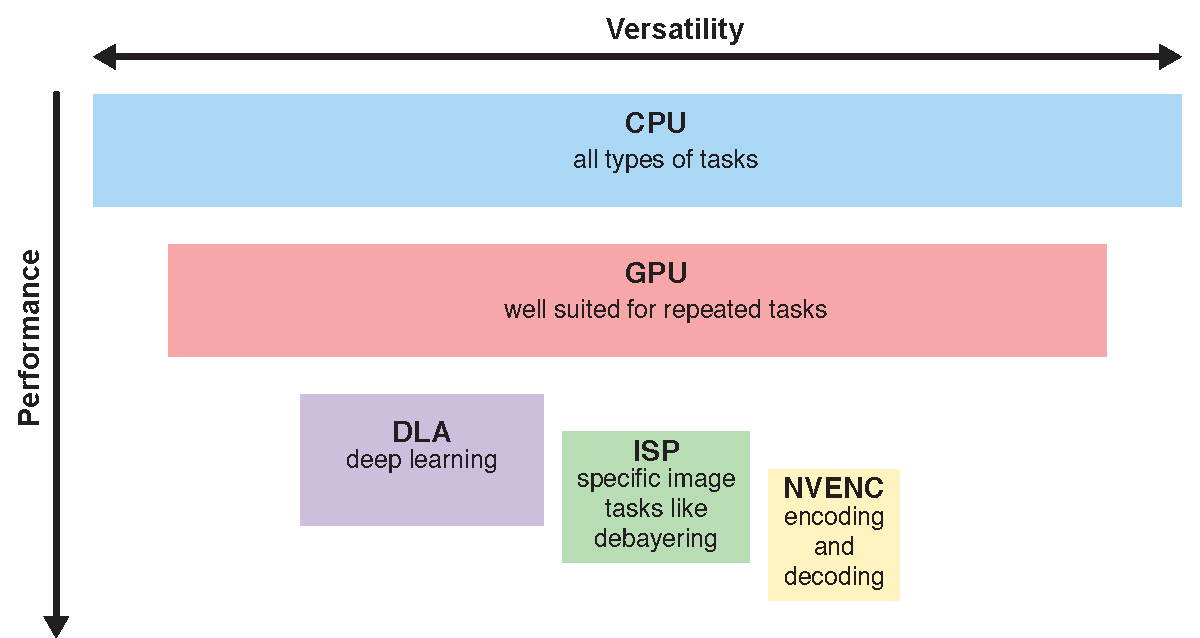
\includegraphics[width=\textwidth]{figures/PDF/jx_hierarchy.pdf}
    \caption{Illustration of the versatility and performance of different types of cores on the \jx.}
    \label{fig:jx_hierarchy}
\end{figure}


\subsubsection{Memory Management}
With different types of cores comes different types of memory.
A key challenge of working with heterogeneous computing systems is to manage the different types of memory efficiently, so that the different cores have access to the data they need when they need it.

A major advantage of working on the \jx is the posibility to share memory between the different types of cores, removing the need for expensive data transfers between the different types of memory.
This is further discussed in Section \ref{sec:jx_memory}.

\begin{figure}
    \centering
    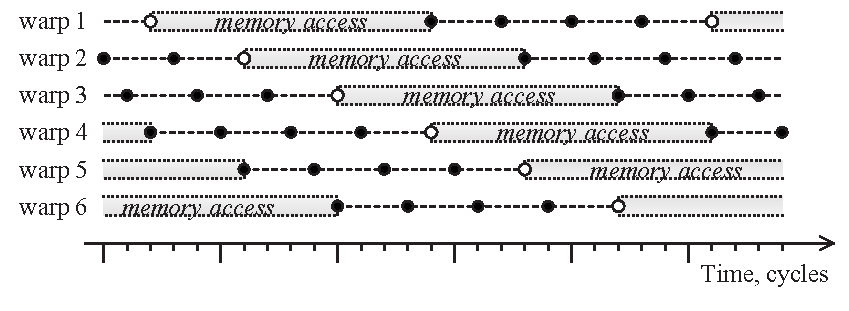
\includegraphics[width=\textwidth]{figures/PDF/concurrency_p54.pdf}
    \caption{Visualization of concurrent execution on a GPU \cite[54]{volkovLatencyHiding2016}}
    \label{fig:concurrency}
\end{figure}


\subsubsection{Latency Hiding}
Latency hiding is a technique used by modern commodity processors such as GPUs to better utilize their numerous execution units and hide execution latencies \cite[35]{volkovLatencyHiding2016}
The idea behind latency hiding is to keep the processor busy with other tasks while it waits for data to be fetched from memory.
This is achieved by executing multiple threads in parallel, so that when one thread is waiting for data, another thread can continue executing.


\subsubsection{Profiling}
Profiling is the process of measuring the performance of a program, and is an important tool for optimizing programs.

In many cases it is straight forward; record the time when a task is started and when it is finished, and calculate the difference.


However, when working with heterogeneous computing systems, it is not always

nsys memory profiling does not work in Pinned Memory

